\begin{section}{Résultats pour l'ensemble des séquences}
Dans cette section, nous présentons les résultats de la qualité visuelle,
mesurée avec le PSNR, obtenus pour chacune des différentes approches de
dissimulation. Ceux-ci sont mesurés en fonction des taux d'erreurs binaires
(BER) 0.0004, 0.0008, 0.0016 et 0.0032 représentant différentes conditions de
diffusion sur un réseau peu fiable. Tout d'abord, pour chaque taux d'erreurs,
nous présentons un tableau qui résume les valeurs moyennes du PSNR de chaque
approche. Par la suite, nous présentons les histogrammes de la distribution du
PSNR pour chaque QP (16, 20, 24, 28). Ces taux et ces QP sont les mêmes que ceux
utilisés au chapitre \ref{chap-resultats} <<~\nameref{chap-resultats}~>>.

% ==============================================================================
% B E R - 0.0004
% ------------------------------------------------------------------------------
% Dispersed
\begin{subsection}{Taux d'erreurs binaires (BER) 0.0004}
\begin{table}
\caption[Résumé des résultats obtenus sur l'ensemble des séquences pour un taux
d'erreurs de 0.0004 (dispersé)]{Résumé des résultats obtenus sur l'ensemble
des séquences pour un taux d'erreurs de 0.0004 (dispersé).}
\centering
\begin{tabular}{| l | c | c | c | c |}
 \hline
 \multirow{2}{*}{\textbf{Approche}} & \multicolumn{4}{c |}{\textbf{PSNR Moyen
 dispersé (dB)}}\\
  \cline{2-5}
 &QP 16 & QP 20 & QP 24 & QP 28 \\ \hline
Encodée (sans erreur) & 45.83& 42.57& 39.59& 36.88\\ \hline
Sélective par bloc (avec référence) & 40.53& 39.20& 38.15&
36.15\\ \hline Sélective par tranche (avec référence)& 39.64& 38.39&
37.59& 35.83\\ \hline Sélective par bloc & \textbf{39.31}&
\textbf{38.06}& \textbf{37.22}& \textbf{35.31}\\ \hline Sélective
par tranche & \textbf{38.94}& \textbf{37.81}& \textbf{37.37}&
\textbf{35.68}\\ \hline Dissimulation tranche calquée & 37.80&
36.87& 35.78& 34.27\\ \hline Trame corrompue & 37.80& 36.87&
35.78& 34.27\\
\hline
\end{tabular}
\end{table}

\begin{figure} \fbox{ \centering
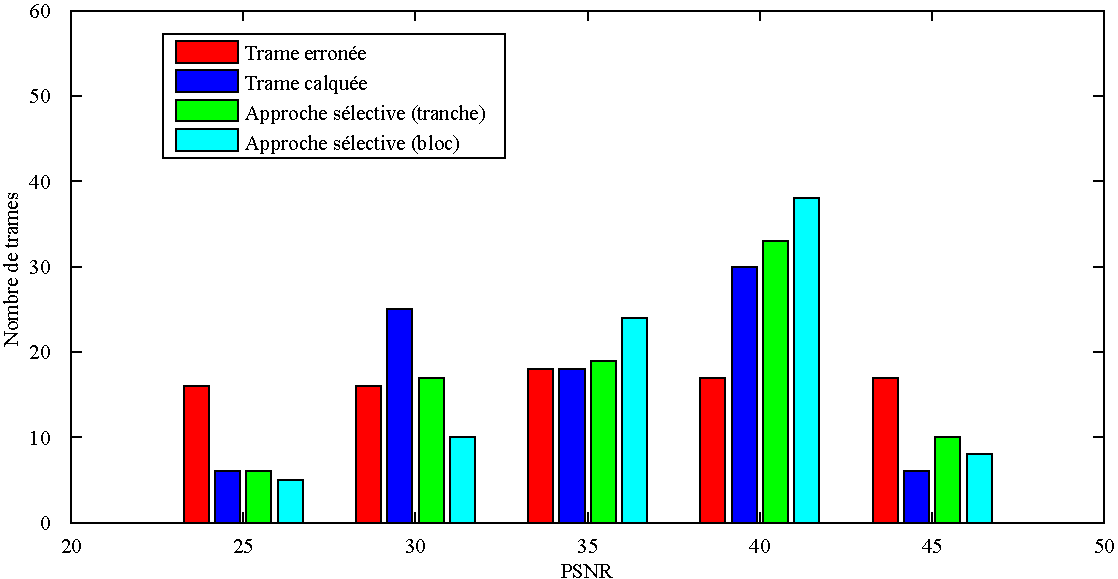
\includegraphics[width=0.97\linewidth]{Annexe/HistAllDispersed16x4.pdf} }
\caption[]{Histogrammes des PSNR des trames, selon l'approche de dissimulation
utilisée. (QP = 16, BER = 0.0004, FMO = Dispersé)}
\label{fig-HistAllDispersed16x4}
\end{figure}

\begin{figure} \fbox{ \centering
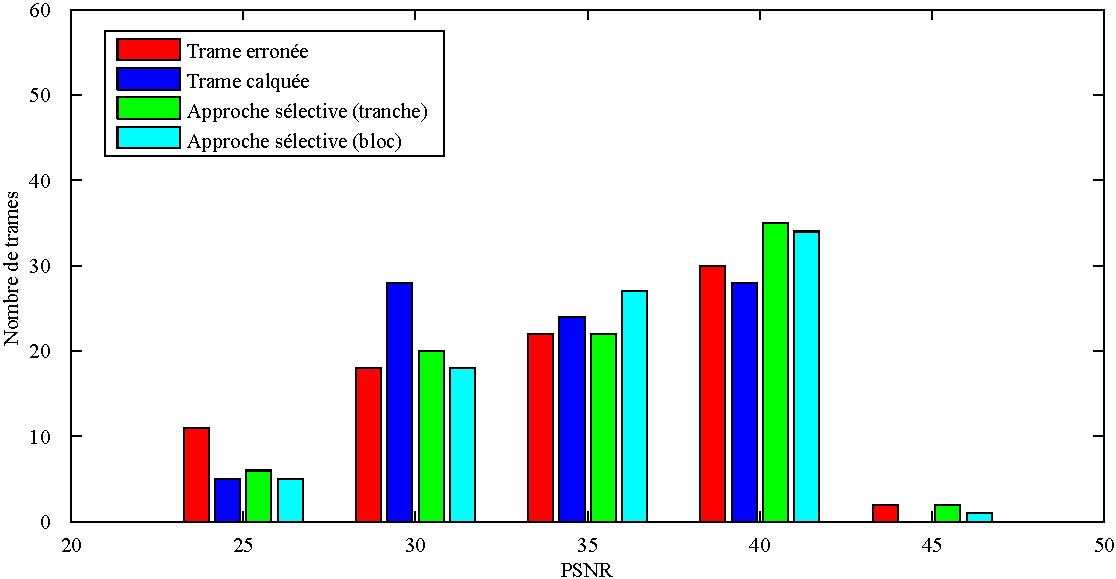
\includegraphics[width=0.97\linewidth]{Annexe/HistAllDispersed20x4.pdf} }
\caption[]{Histogrammes des PSNR des trames, selon l'approche de dissimulation
utilisée. (QP = 20, BER = 0.0004, FMO = Dispersé)}
\label{fig-HistAllDispersed20x4}
\end{figure}

\begin{figure} \fbox{ \centering
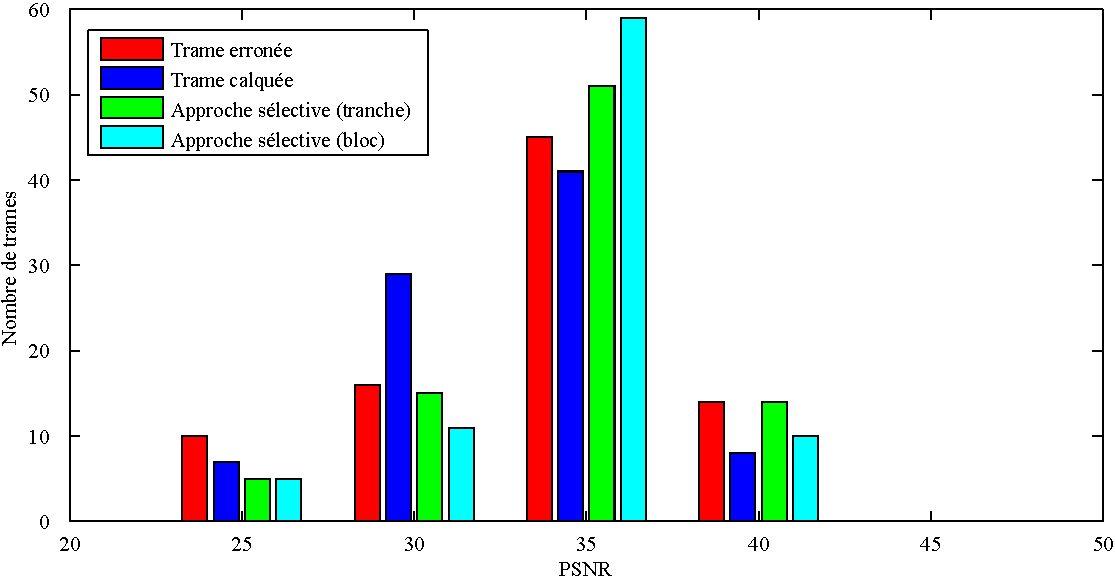
\includegraphics[width=0.97\linewidth]{Annexe/HistAllDispersed24x4.pdf} }
\caption[]{Histogrammes des PSNR des trames, selon l'approche de dissimulation
utilisée. (QP = 24, BER = 0.0004, FMO = Dispersé)}
\label{fig-HistAllDispersed24x4}
\end{figure}

\begin{figure} \fbox{ \centering
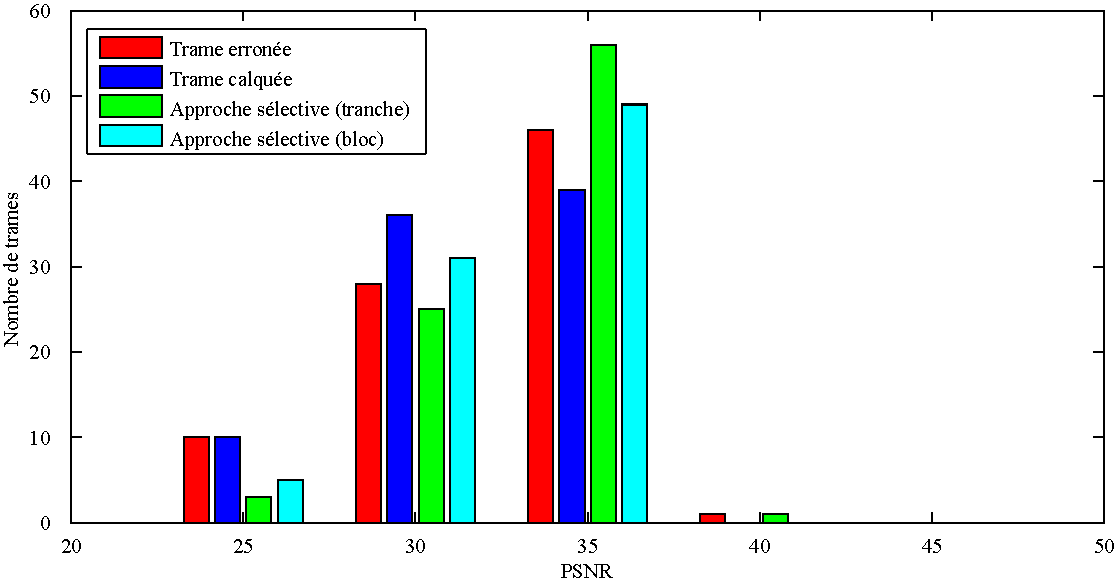
\includegraphics[width=0.97\linewidth]{Annexe/HistAllDispersed28x4.pdf} }
\caption[]{Histogrammes des PSNR des trames, selon l'approche de dissimulation
utilisée. (QP = 28, BER = 0.0004, FMO = Dispersé)}
\label{fig-HistAllDispersed28x4}
\end{figure}
\FloatBarrier

% ------------------------------------------------------------------------------
% Interleaved
\begin{table}
\caption[Résumé des résultats obtenus sur l'ensemble des séquences pour un taux
d'erreurs de 0.0004 (entrelacé)]{Résumé des résultats obtenus sur l'ensemble des
séquences pour un taux d'erreurs de 0.0004 (entrelacé).}
\centering
\begin{tabular}{| l | c | c | c | c |}
 \hline
 \multirow{2}{*}{\textbf{Approche}} & \multicolumn{4}{c |}{\textbf{PSNR Moyen
 entrelacé (dB)}}\\
  \cline{2-5}
 &QP 16 & QP 20 & QP 24 & QP 28 \\ \hline
Encodée (sans erreur) & 45.83& 42.56& 39.56& 36.85\\ \hline
Sélective par bloc (avec référence) & 42.19& 40.55& 38.59&
36.22\\ \hline Sélective par tranche (avec référence)& 41.63& 39.91&
38.20& 35.91\\ \hline Sélective par bloc & \textbf{40.86}&
\textbf{39.51}& \textbf{37.98}& \textbf{35.79}\\ \hline Sélective
par tranche & \textbf{41.46}& \textbf{39.75}& \textbf{38.15}&
\textbf{35.76}\\ \hline Dissimulation tranche calquée & 39.26&
38.14& 36.72& 34.94\\ \hline Trame corrompue & 39.26& 38.14&
36.72& 34.94\\
\hline
\end{tabular}
\end{table}

\begin{figure} \fbox{ \centering
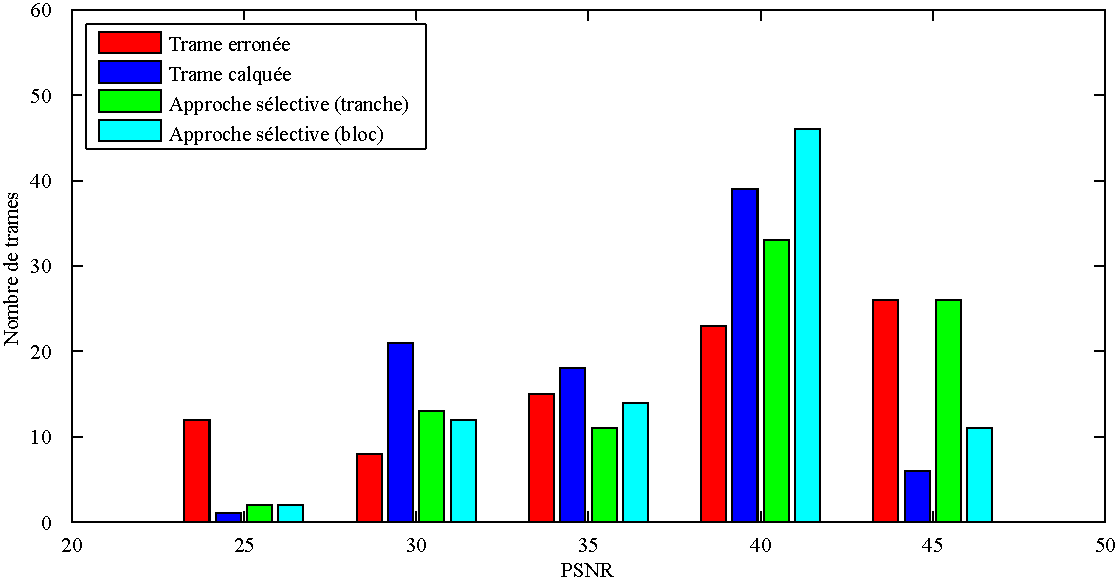
\includegraphics[width=0.97\linewidth]{Annexe/HistAllInterleaved16x4.pdf} }
\caption[]{Histogrammes des PSNR des trames, selon l'approche de dissimulation
utilisée. (QP = 16, BER = 0.0004, FMO = Entrelacé)}
\label{fig-HistAllDInterlaced16x4}
\end{figure}

\begin{figure} \fbox{ \centering
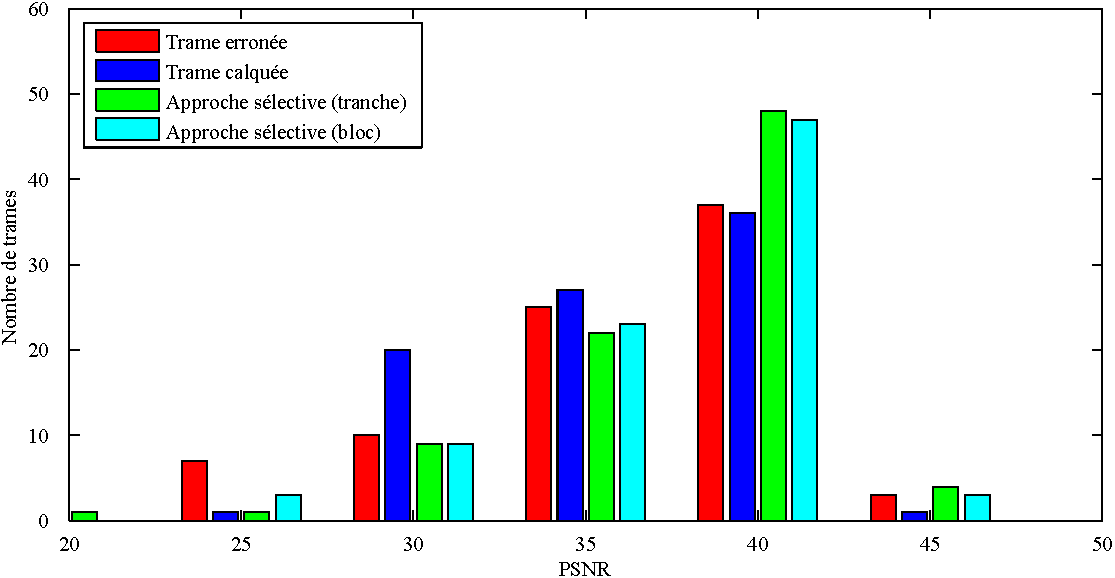
\includegraphics[width=0.97\linewidth]{Annexe/HistAllInterleaved20x4.pdf} }
\caption[]{Histogrammes des PSNR des trames, selon l'approche de dissimulation
utilisée. (QP = 20, BER = 0.0004, FMO = Entrelacé)}
\label{fig-HistAllDInterlaced20x4}
\end{figure}

\begin{figure} \fbox{ \centering
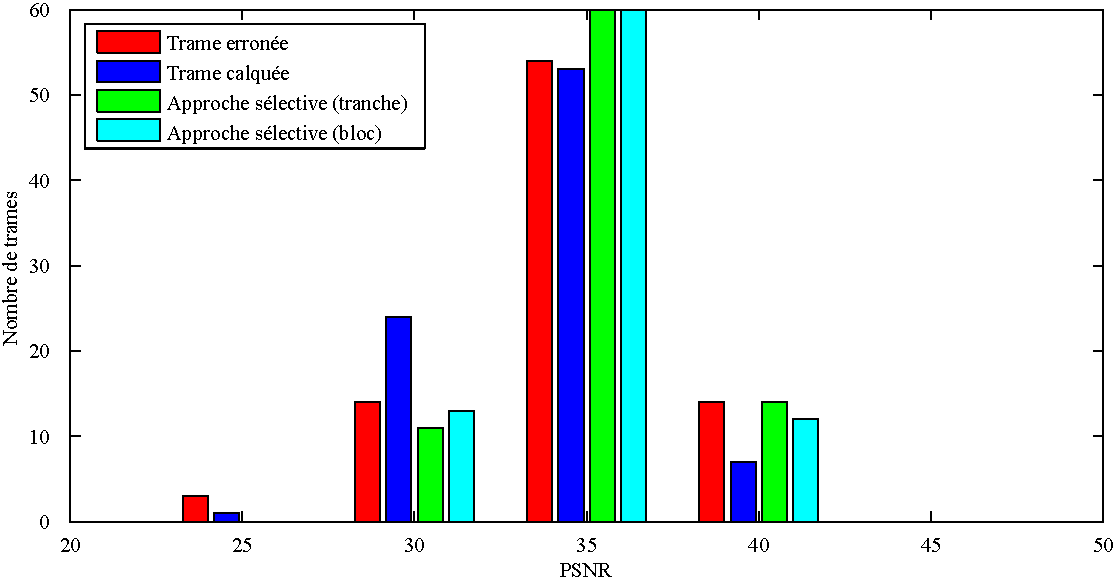
\includegraphics[width=0.97\linewidth]{Annexe/HistAllInterleaved24x4.pdf} }
\caption[]{Histogrammes des PSNR des trames, selon l'approche de dissimulation
utilisée. (QP = 24, BER = 0.0004, FMO = Entrelacé)}
\label{fig-HistAllDInterlaced24x4}
\end{figure}

\begin{figure} \fbox{ \centering
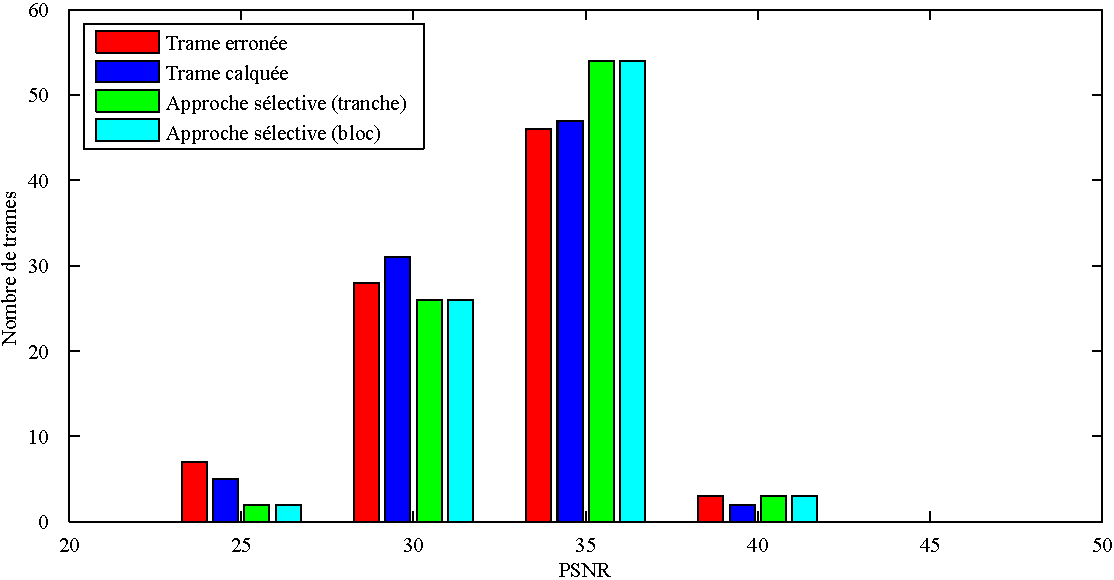
\includegraphics[width=0.97\linewidth]{Annexe/HistAllInterleaved28x4.pdf} }
\caption[]{Histogrammes des PSNR des trames, selon l'approche de dissimulation
utilisée. (QP = 28, BER = 0.0004, FMO = Entrelacé)}
\label{fig-HistAllDInterlaced28x4}
\end{figure}

\FloatBarrier
\end{subsection}
% ==============================================================================

% ==============================================================================
% B E R - 0.0008
% ------------------------------------------------------------------------------
% Dispersed
\begin{subsection}{Taux d'erreurs binaires (BER) 0.0008}
\begin{table}
\caption[Résumé des résultats obtenus sur l'ensemble des séquences pour un taux
d'erreurs de 0.0008 (dispersé)]{Résumé des résultats obtenus sur l'ensemble des
séquences pour un taux d'erreurs de 0.0008 (dispersé).}
\centering
\begin{tabular}{| l | c | c | c | c |}
 \hline
 \multirow{2}{*}{\textbf{Approche}} & \multicolumn{4}{c |}{\textbf{PSNR Moyen
 dispersé (dB)}}\\
  \cline{2-5}
 &QP 16 & QP 20 & QP 24 & QP 28 \\ \hline
Encodée (sans erreur) & 45.83& 42.57& 39.59& 36.88\\ \hline
Sélective par bloc (avec référence) & 39.44& 39.07& 37.67&
35.94\\ \hline Sélective par tranche (avec référence)& 38.75& 38.27&
36.99& 35.42\\ \hline Sélective par bloc & \textbf{38.75}&
\textbf{38.19}& \textbf{36.83}& \textbf{35.20}\\ \hline Sélective
par tranche & \textbf{38.37}& \textbf{37.98}& \textbf{36.84}&
\textbf{35.32}\\ \hline Dissimulation tranche calquée & 37.80&
36.87& 35.78& 34.27\\ \hline Trame corrompue & 37.80& 36.87&
35.78& 34.27\\ \hline
\end{tabular}
\end{table}

\begin{figure} \fbox{ \centering
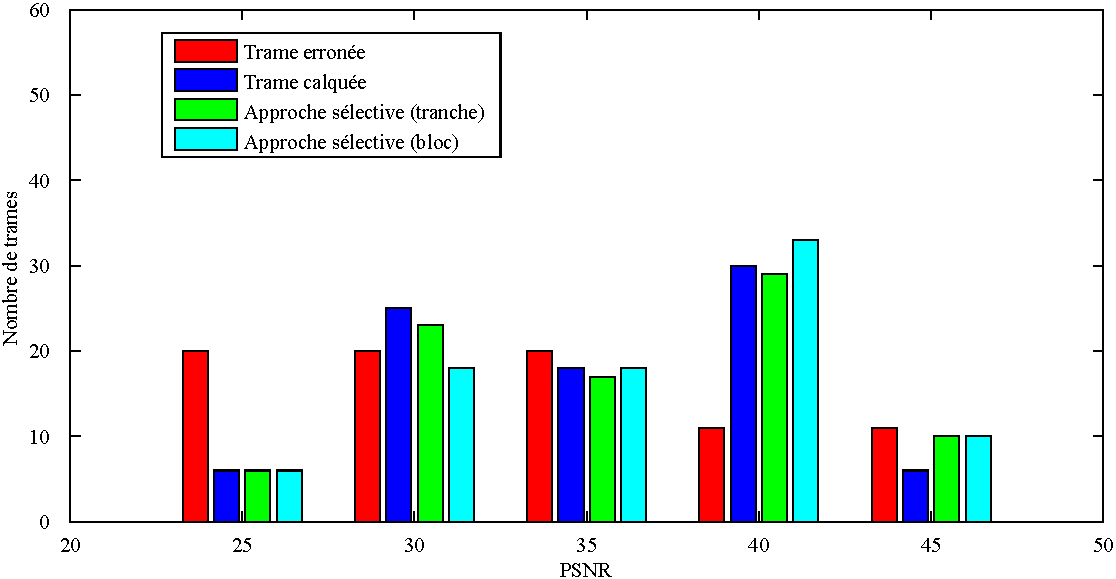
\includegraphics[width=0.97\linewidth]{Annexe/HistAllDispersed16x8.pdf} }
\caption[]{Histogrammes des PSNR des trames, selon l'approche de dissimulation
utilisée. (QP = 16, BER = 0.0008, FMO = Dispersé)}
\label{fig-HistAllDispersed16x8}
\end{figure}

\begin{figure} \fbox{ \centering
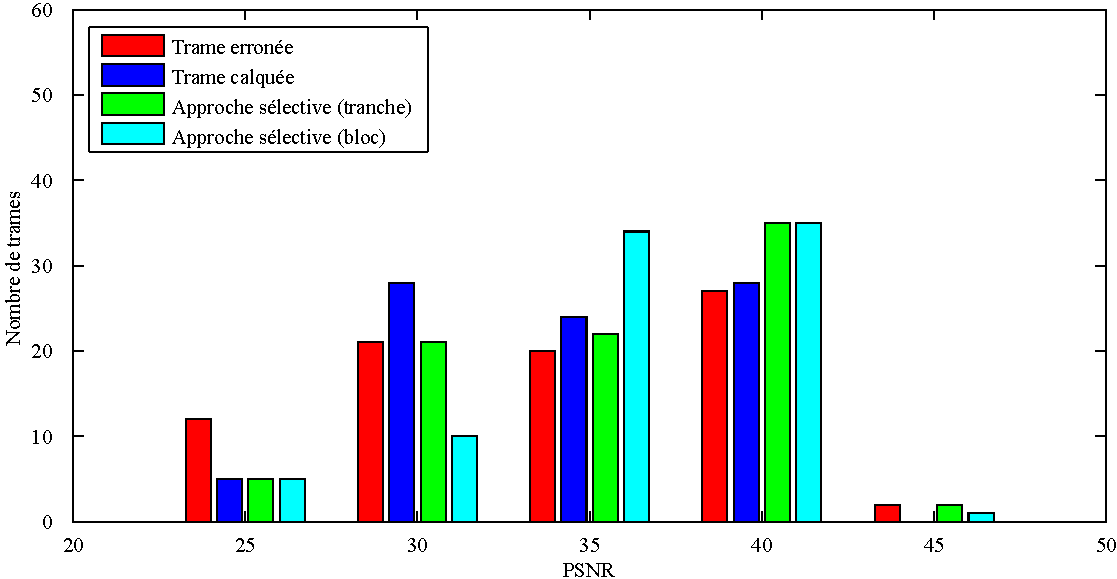
\includegraphics[width=0.97\linewidth]{Annexe/HistAllDispersed20x8.pdf} }
\caption[]{Histogrammes des PSNR des trames, selon l'approche de dissimulation
utilisée. (QP = 20, BER = 0.0008, FMO = Dispersé)}
\label{fig-HistAllDispersed20x8}
\end{figure}

\begin{figure} \fbox{ \centering
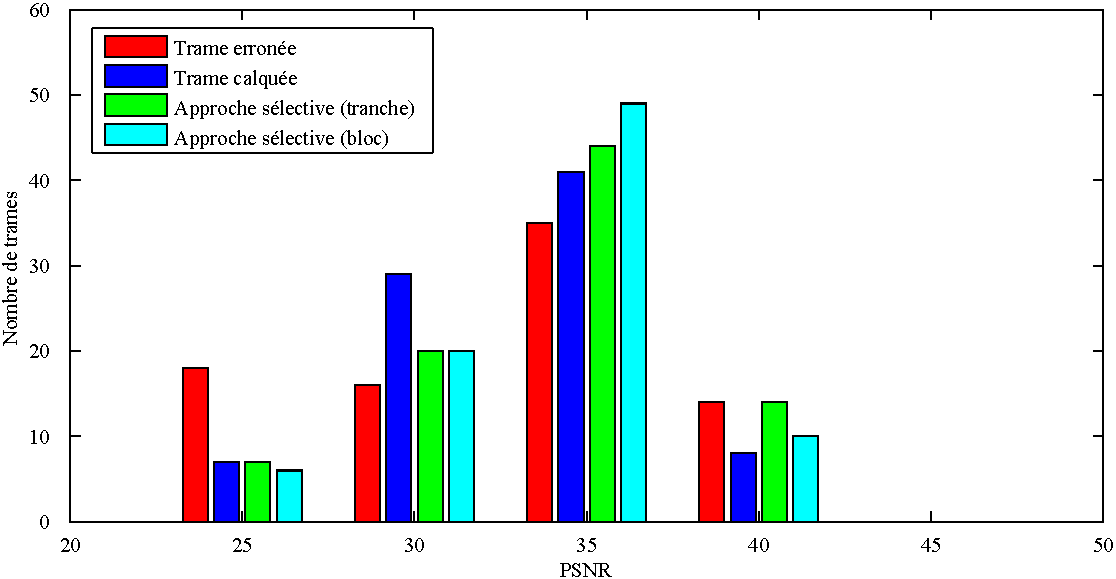
\includegraphics[width=0.97\linewidth]{Annexe/HistAllDispersed24x8.pdf} }
\caption[]{Histogrammes des PSNR des trames, selon l'approche de dissimulation
utilisée. (QP = 24, BER = 0.0008, FMO = Dispersé)}
\label{fig-HistAllDispersed24x8}
\end{figure}

\begin{figure} \fbox{ \centering
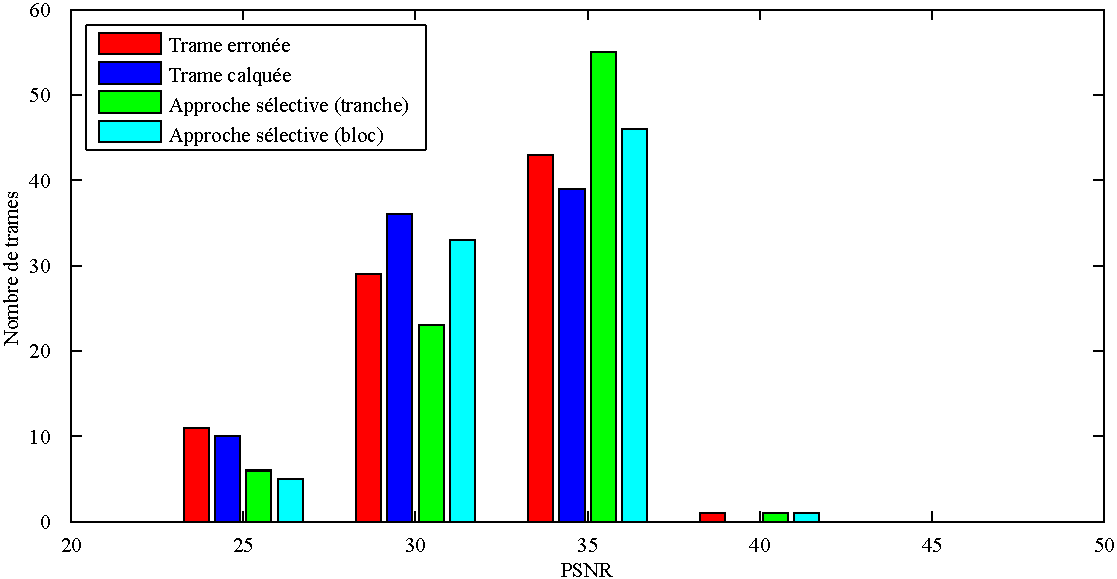
\includegraphics[width=0.97\linewidth]{Annexe/HistAllDispersed28x8.pdf} }
\caption[]{Histogrammes des PSNR des trames, selon l'approche de dissimulation
utilisée. (QP = 28, BER = 0.0008, FMO = Dispersé)}
\label{fig-HistAllDispersed28x8}
\end{figure}

\FloatBarrier
% ------------------------------------------------------------------------------
% Interleaved

\begin{table}
\caption[Résumé des résultats obtenus sur l'ensemble des séquences pour un taux
d'erreurs de 0.0008 (entrelacé)]{Résumé des résultats obtenus sur l'ensemble des
séquences pour un taux d'erreurs de 0.0008 (entrelacé).}
\centering
\begin{tabular}{| l | c | c | c | c |}
 \hline
 \multirow{2}{*}{\textbf{Approche}} & \multicolumn{4}{c |}{\textbf{PSNR Moyen
 entrelacé (dB)}}\\
  \cline{2-5}
   &QP 16 & QP 20 & QP 24 & QP 28 \\ \hline
Encodée (sans erreur) & 45.83& 42.56& 39.56& 36.85\\ \hline Sélective par bloc
(avec référence) & 40.78& 39.60& 38.10& 36.13\\ \hline Sélective par tranche
(avec référence)& 40.02& 38.99& 37.65& 35.83\\ \hline Sélective par bloc &
\textbf{39.97}& \textbf{38.96}& \textbf{37.59}& \textbf{35.66}\\ \hline
Sélective par tranche & \textbf{39.78}& \textbf{38.83}& \textbf{37.47}&
\textbf{35.69}\\ \hline Dissimulation tranche calquée & 39.26& 38.14&
36.72& 34.94\\ \hline Trame corrompue & 39.26& 38.14& 36.72& 34.94\\
\hline
\end{tabular}
\end{table}

\begin{figure} \fbox{ \centering
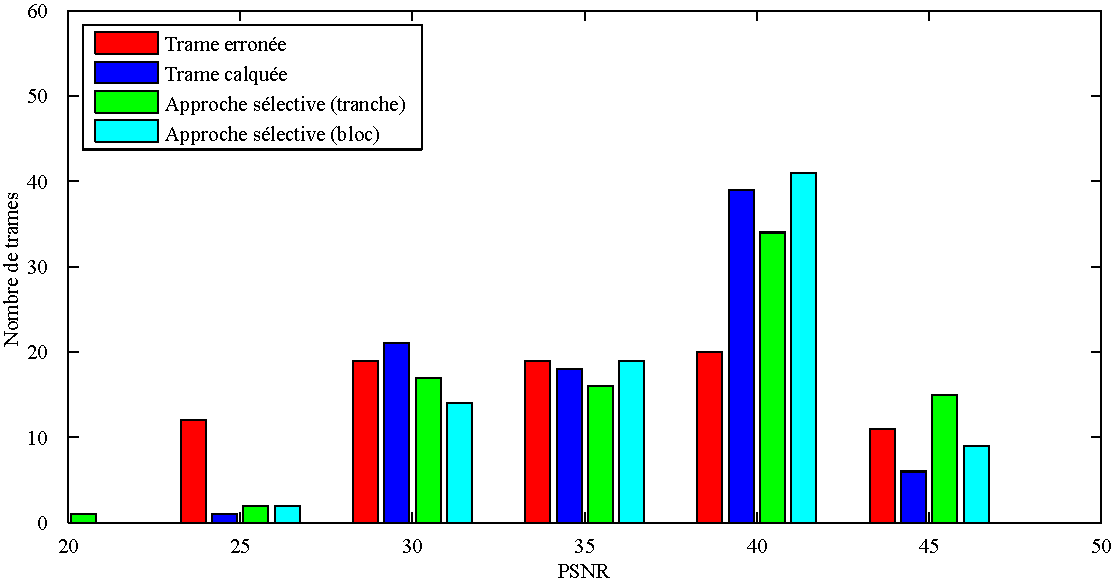
\includegraphics[width=0.97\linewidth]{Annexe/HistAllInterleaved16x8.pdf} }
\caption[]{Histogrammes des PSNR des trames, selon l'approche de dissimulation
utilisée. (QP = 16, BER = 0.0008, FMO = Entrelacé)}
\label{fig-HistAllDInterlaced16x8}
\end{figure}

\begin{figure} \fbox{ \centering
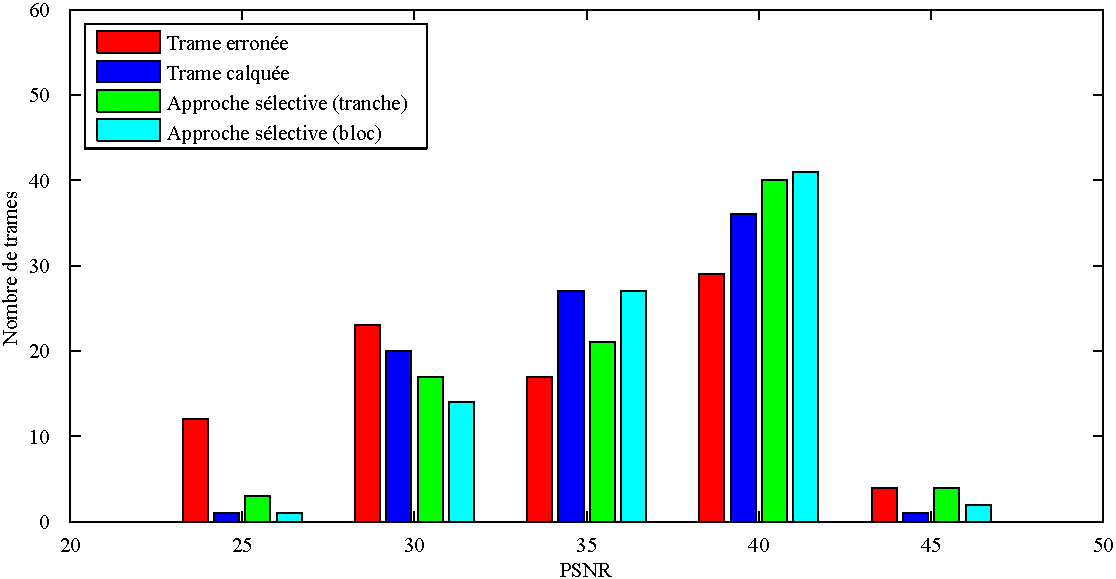
\includegraphics[width=0.97\linewidth]{Annexe/HistAllInterleaved20x8.pdf} }
\caption[]{Histogrammes des PSNR des trames, selon l'approche de dissimulation
utilisée. (QP = 20, BER = 0.0008, FMO = Entrelacé)}
\label{fig-HistAllDInterlaced20x8}
\end{figure}

\begin{figure} \fbox{ \centering
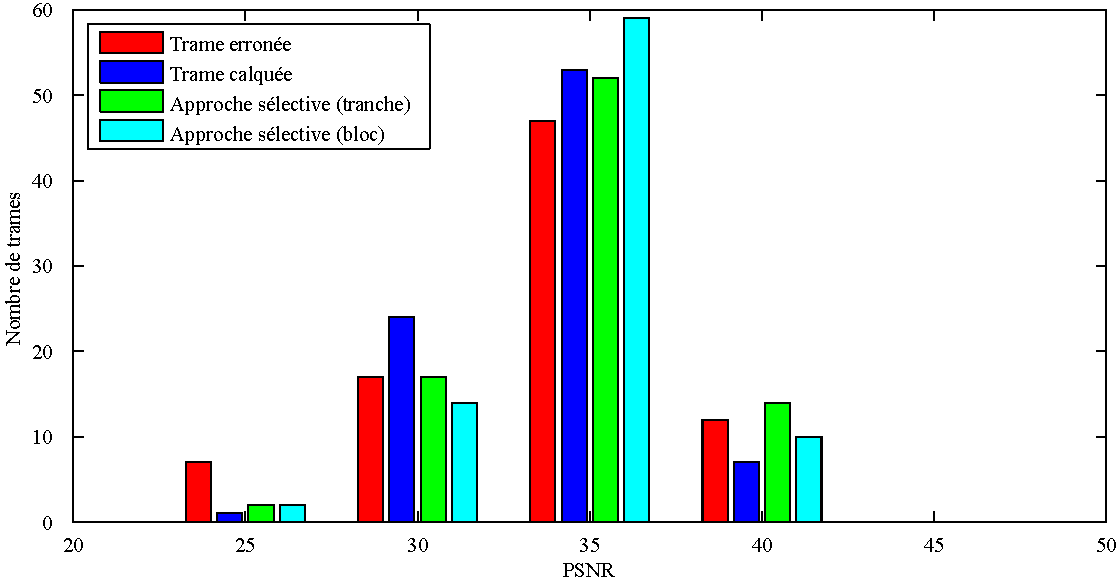
\includegraphics[width=0.97\linewidth]{Annexe/HistAllInterleaved24x8.pdf} }
\caption[]{Histogrammes des PSNR des trames, selon l'approche de dissimulation
utilisée. (QP = 24, BER = 0.0008, FMO = Entrelacé)}
\label{fig-HistAllDInterlaced24x8}
\end{figure}

\begin{figure} \fbox{ \centering
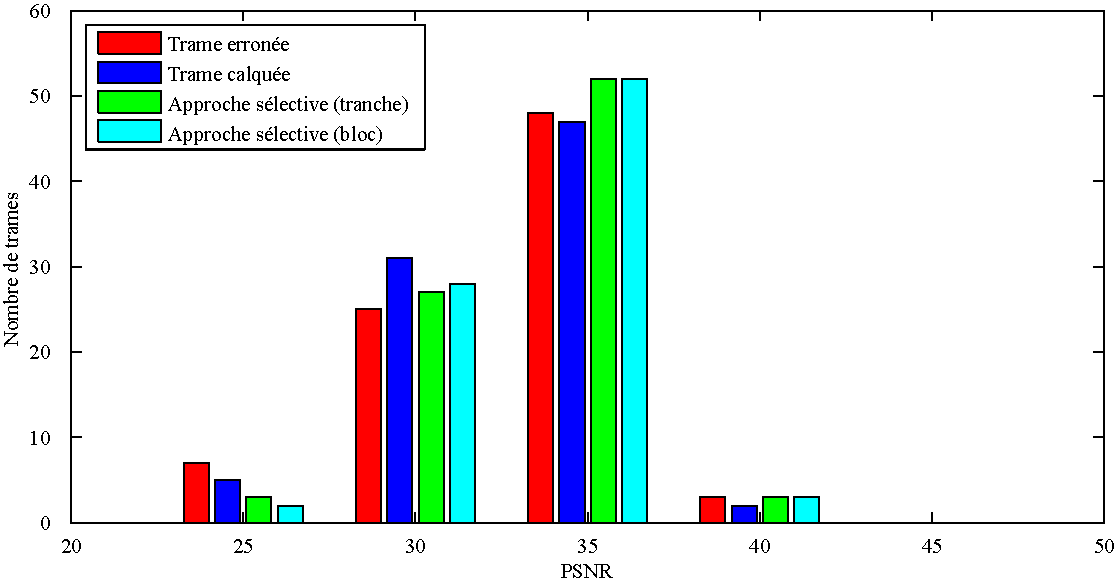
\includegraphics[width=0.97\linewidth]{Annexe/HistAllInterleaved28x8.pdf} }
\caption[]{Histogrammes des PSNR des trames, selon l'approche de dissimulation
utilisée. (QP = 28, BER = 0.0008, FMO = Entrelacé)}
\label{fig-HistAllDInterlaced28x8}
\end{figure}

\FloatBarrier
\end{subsection}
% ==============================================================================

% ==============================================================================
% B E R - 0.0016
% ------------------------------------------------------------------------------
% Dispersed
\begin{subsection}{Taux d'erreurs binaires (BER) 0.0016}
\begin{table}
\caption[Résumé des résultats obtenus sur l'ensemble des séquences pour un taux
d'erreurs de 0.0016 (dispersé)]{Résumé des résultats obtenus sur l'ensemble des
séquences pour un taux d'erreurs de 0.0016 (dispersé).}
\centering
\begin{tabular}{| l | c | c | c | c |}
 \hline
 \multirow{2}{*}{\textbf{Approche}} & \multicolumn{4}{c |}{\textbf{PSNR Moyen
 dispersé (dB)}}\\
  \cline{2-5}
   &QP 16 & QP 20 & QP 24 & QP 28 \\ \hline
Encodée (sans erreur) & 45.83& 42.57& 39.59& 36.88\\ \hline
Sélective par bloc (avec référence) & 38.47& 38.10& 37.10& 35.66\\
\hline Sélective par tranche (avec référence)& 37.96& 37.46& 36.45&
35.28\\ \hline Sélective par bloc & \textbf{38.12}& \textbf{37.61}&
\textbf{36.53}& \textbf{35.13}\\ \hline Sélective par tranche & \textbf{37.92}&
\textbf{37.30}& \textbf{36.21}& \textbf{35.25}\\ \hline Dissimulation
tranche calquée & 37.80& 36.87& 35.78& 34.27\\ \hline Trame corrompue &
37.80& 36.88& 35.78& 34.27\\
\hline
\end{tabular}
\end{table}

\begin{figure} \fbox{ \centering
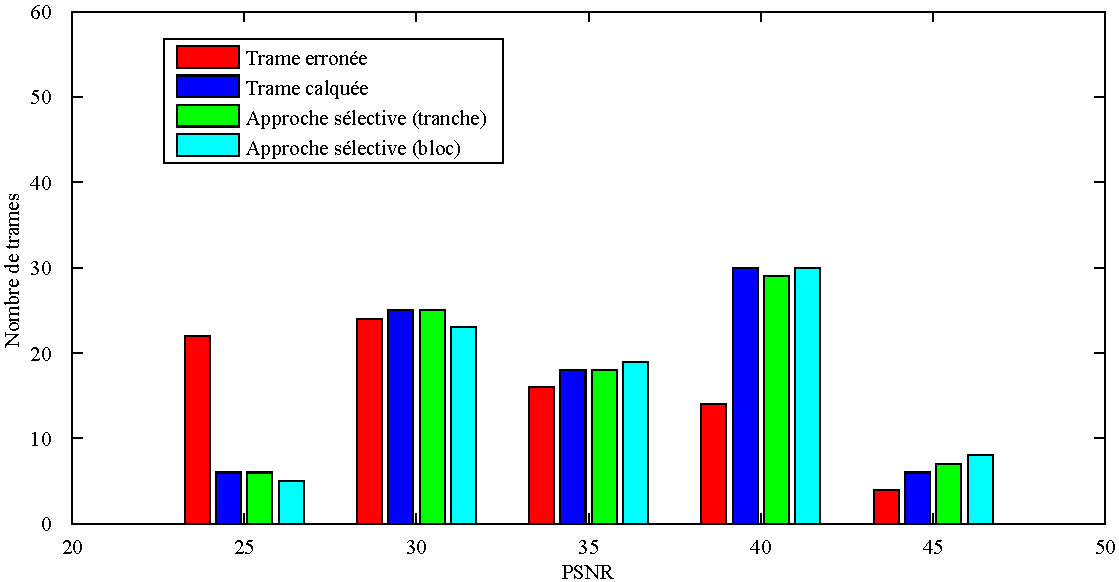
\includegraphics[width=0.97\linewidth]{Annexe/HistAllDispersed16x16.pdf} }
\caption[]{Histogrammes des PSNR des trames, selon l'approche de dissimulation
utilisée. (QP = 16, BER = 0.0016, FMO = Dispersé)}
\label{fig-HistAllDispersed16x16}
\end{figure}

\begin{figure} \fbox{ \centering
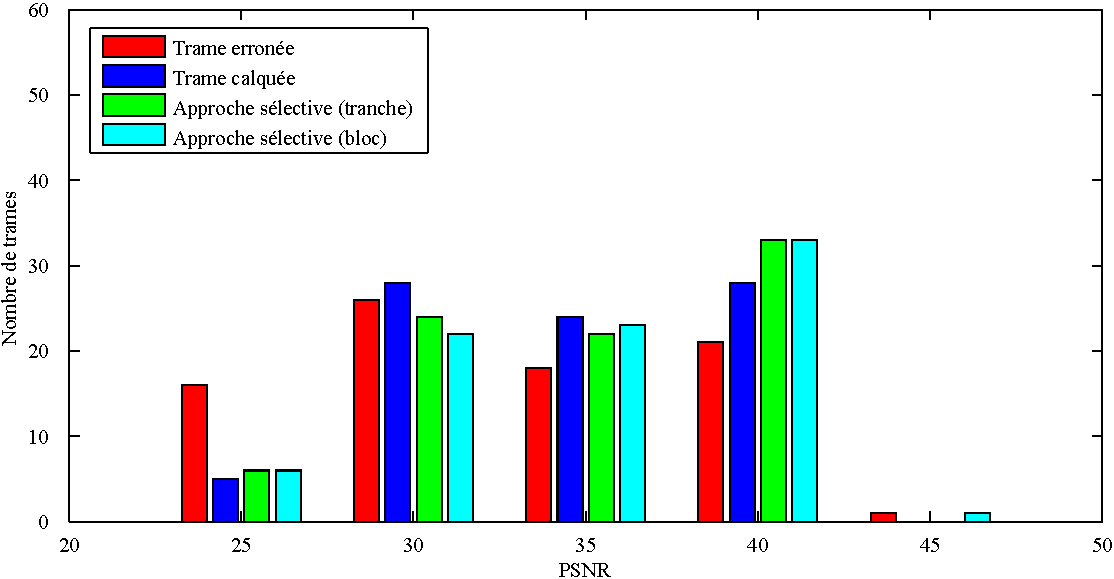
\includegraphics[width=0.97\linewidth]{Annexe/HistAllDispersed20x16.pdf} }
\caption[]{Histogrammes des PSNR des trames, selon l'approche de dissimulation
utilisée. (QP = 20, BER = 0.0016, FMO = Dispersé)}
\label{fig-HistAllDispersed20x16}
\end{figure}

\begin{figure} \fbox{ \centering
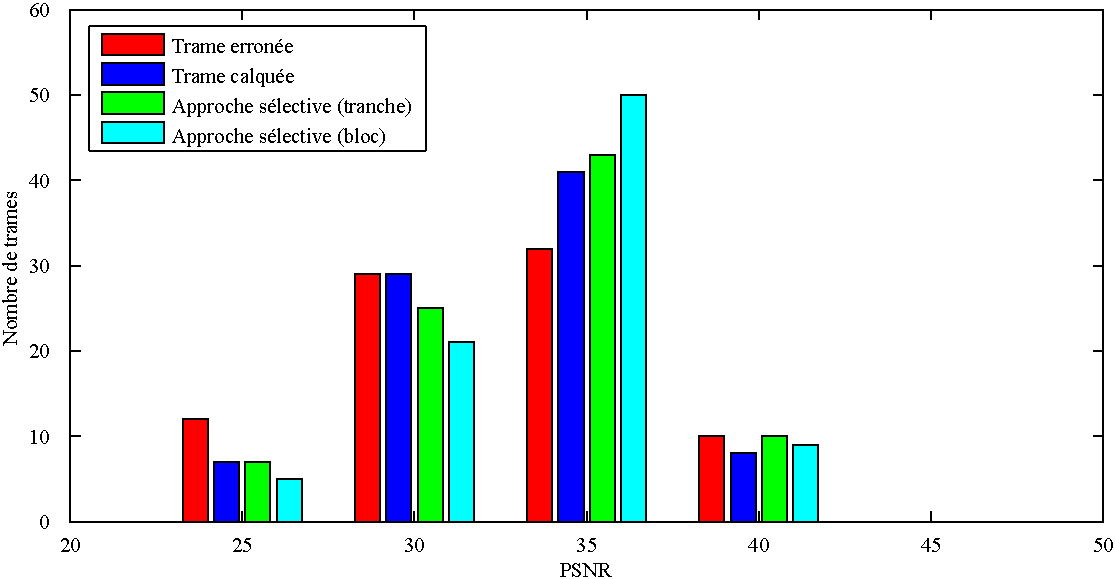
\includegraphics[width=0.97\linewidth]{Annexe/HistAllDispersed24x16.pdf} }
\caption[]{Histogrammes des PSNR des trames, selon l'approche de dissimulation
utilisée. (QP = 24, BER = 0.0016, FMO = Dispersé)}
\label{fig-HistAllDispersed24x8}
\end{figure}

\begin{figure} \fbox{ \centering
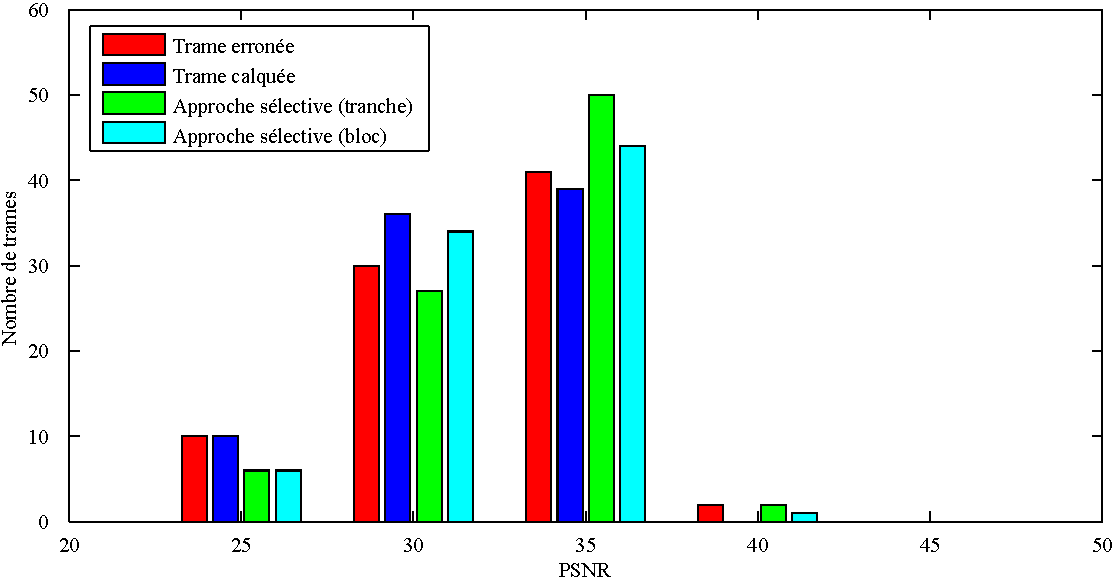
\includegraphics[width=0.97\linewidth]{Annexe/HistAllDispersed28x16.pdf} }
\caption[]{Histogrammes des PSNR des trames, selon l'approche de dissimulation
utilisée. (QP = 28, BER = 0.0016, FMO = Dispersé)}
\label{fig-HistAllDispersed28x8}
\end{figure}

\FloatBarrier
% ------------------------------------------------------------------------------
% Interleaved

\begin{table}
\caption[Résumé des résultats obtenus sur l'ensemble des séquences pour un taux
d'erreurs de 0.0016 (entrelacé)]{Résumé des résultats obtenus sur l'ensemble des
séquences pour un taux d'erreurs de 0.0016 (entrelacé).}
\centering
\begin{tabular}{| l | c | c | c | c |}
 \hline
 \multirow{2}{*}{\textbf{Approche}} & \multicolumn{4}{c |}{\textbf{PSNR Moyen
 entrelacé (dB)}}\\
  \cline{2-5}
   &QP 16 & QP 20 & QP 24 & QP 28 \\ \hline
Encodée (sans erreur) & 45.83& 42.56& 39.56& 36.85\\ \hline
Sélective par bloc (avec référence) & 40.22& 39.13& 37.68& 35.94\\
\hline Sélective par tranche (avec référence)& 39.73& 38.62& 37.31& 35.52\\
\hline Sélective par bloc & \textbf{39.67}& \textbf{38.59}&
\textbf{37.24}& \textbf{35.54}\\ \hline Sélective par tranche &
\textbf{39.57}& \textbf{38.43}& \textbf{37.13}& \textbf{35.27}\\ \hline
Dissimulation tranche calquée & 39.26& 38.14& 36.72& 34.94\\ \hline
Trame corrompue & 39.26& 38.14& 36.72& 34.94\\
\hline
\end{tabular}
\end{table}

\begin{figure} \fbox{ \centering
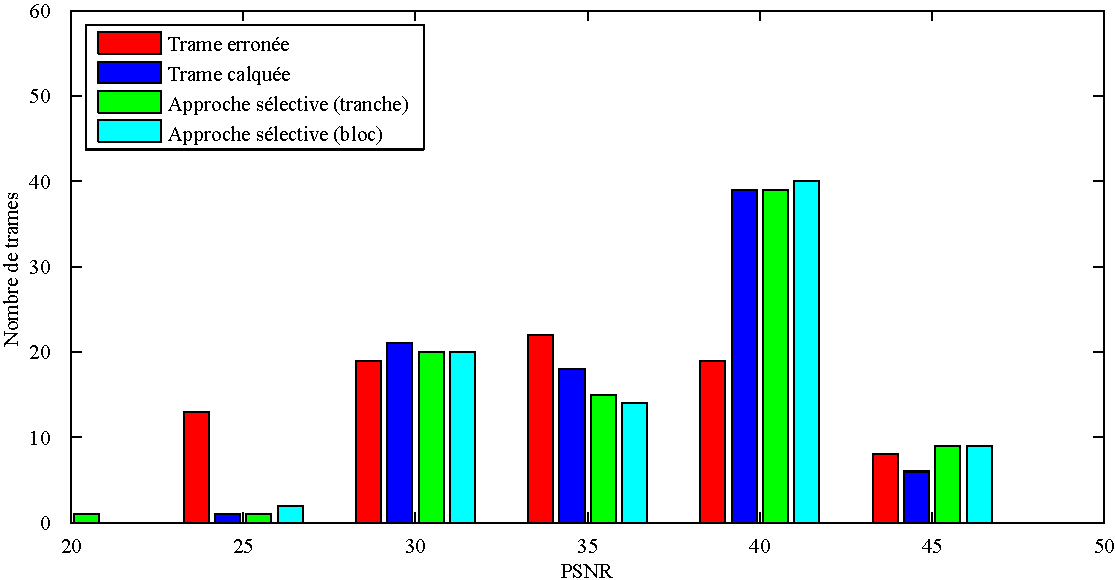
\includegraphics[width=0.97\linewidth]{Annexe/HistAllInterleaved16x16.pdf} }
\caption[]{Histogrammes des PSNR des trames, selon l'approche de dissimulation
utilisée. (QP = 16, BER = 0.0016, FMO = Entrelacé)}
\label{fig-HistAllDInterlaced16x16}
\end{figure}

\begin{figure} \fbox{ \centering
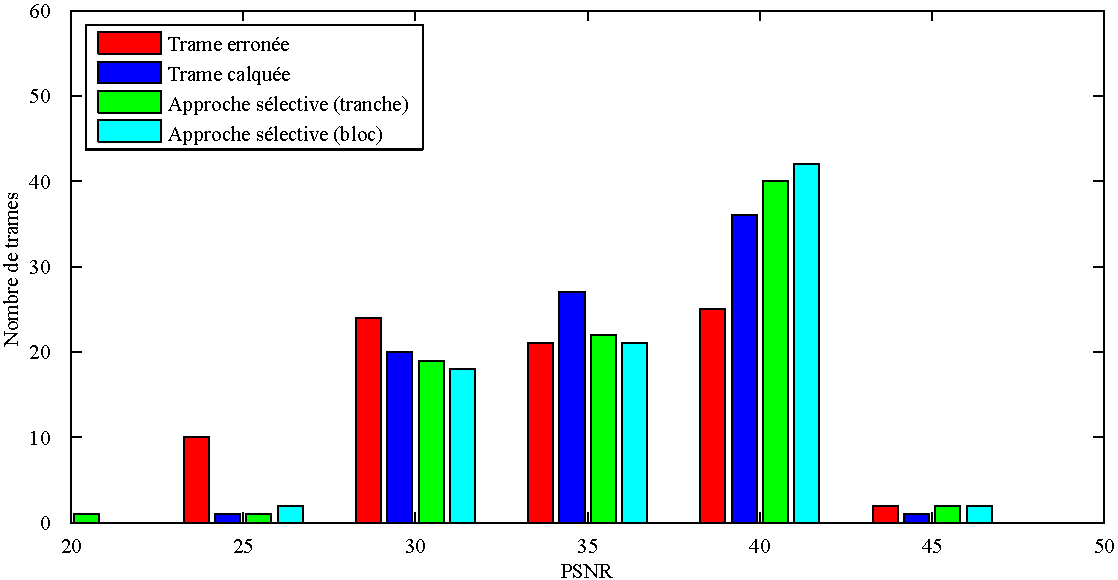
\includegraphics[width=0.97\linewidth]{Annexe/HistAllInterleaved20x16.pdf} }
\caption[]{Histogrammes des PSNR des trames, selon l'approche de dissimulation
utilisée. (QP = 20, BER = 0.0016, FMO = Entrelacé)}
\label{fig-HistAllDInterlaced20x16}
\end{figure}

\begin{figure} \fbox{ \centering
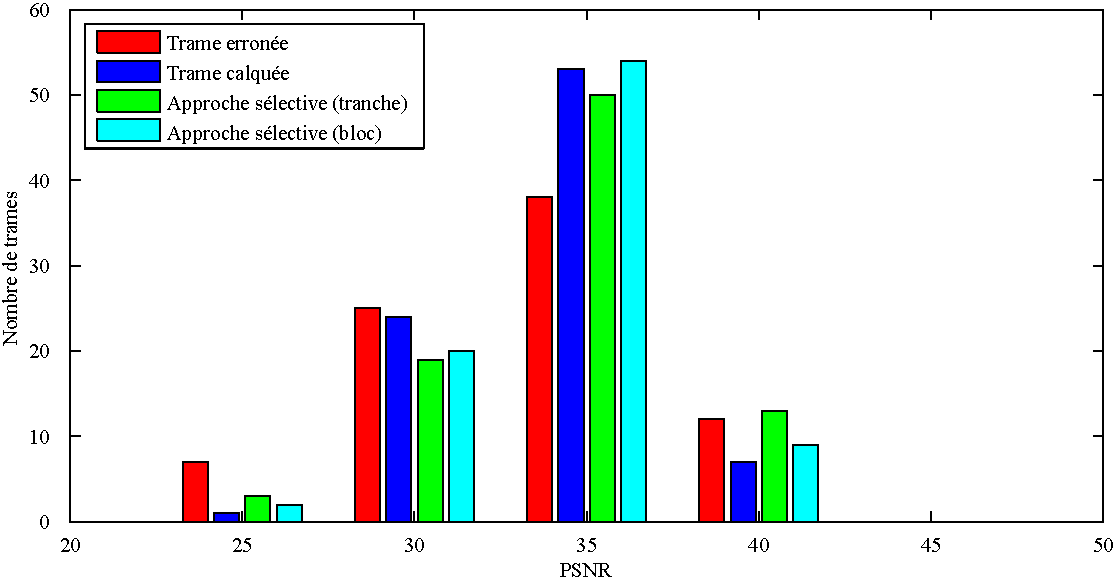
\includegraphics[width=0.97\linewidth]{Annexe/HistAllInterleaved24x16.pdf} }
\caption[]{Histogrammes des PSNR des trames, selon l'approche de dissimulation
utilisée. (QP = 24, BER = 0.0016, FMO = Entrelacé)}
\label{fig-HistAllDInterlaced24x16}
\end{figure}

\begin{figure} \fbox{ \centering
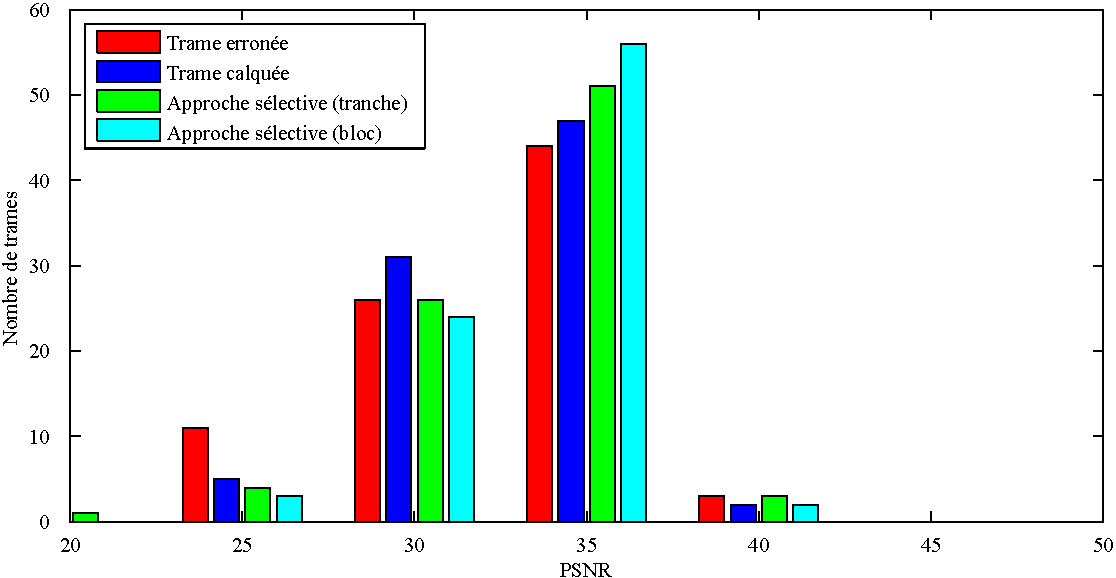
\includegraphics[width=0.97\linewidth]{Annexe/HistAllInterleaved28x16.pdf} }
\caption[]{Histogrammes des PSNR des trames, selon l'approche de dissimulation
utilisée. (QP = 28, BER = 0.0016, FMO = Entrelacé)}
\label{fig-HistAllDInterlaced28x16}
\end{figure}

\FloatBarrier
\end{subsection}
% ==============================================================================

% ==============================================================================
% B E R - 0.0032
% ------------------------------------------------------------------------------
% Dispersed

\begin{subsection}{Taux d'erreurs binaires (BER) 0.0032}
\begin{table}
\caption[Résumé des résultats obtenus sur l'ensemble des séquences pour un taux
d'erreurs de 0.0032 (dispersé)]{Résumé des résultats obtenus sur l'ensemble des
séquences pour un taux d'erreurs de 0.0032 (dispersé).}
\centering
\begin{tabular}{| l | c | c | c | c |}
 \hline
 \multirow{2}{*}{\textbf{Approche}} & \multicolumn{4}{c |}{\textbf{PSNR Moyen
 dispersé (dB)}}\\
  \cline{2-5}
   &QP 16 & QP 20 & QP 24 & QP 28 \\ \hline
Encodée (sans erreur) & 45.83& 42.57& 39.59& 36.88\\ \hline
Sélective par bloc (avec référence) & 38.32& 37.50& 36.68& 35.07\\
\hline Sélective par tranche (avec référence)& 37.95& 37.01& 36.24& 34.66\\
\hline Sélective par bloc & \textbf{38.10}& \textbf{37.22}& \textbf{36.23}&
\textbf{34.69}\\ \hline Sélective par tranche & \textbf{37.90}&
\textbf{36.95}& \textbf{36.04}& \textbf{34.55}\\ \hline Dissimulation
tranche calquée & 37.80& 36.87& 35.78& 34.27\\ \hline Trame corrompue &
37.80& 36.87& 35.78& 34.27\\
\hline
\end{tabular}
\end{table}

\begin{figure} \fbox{ \centering
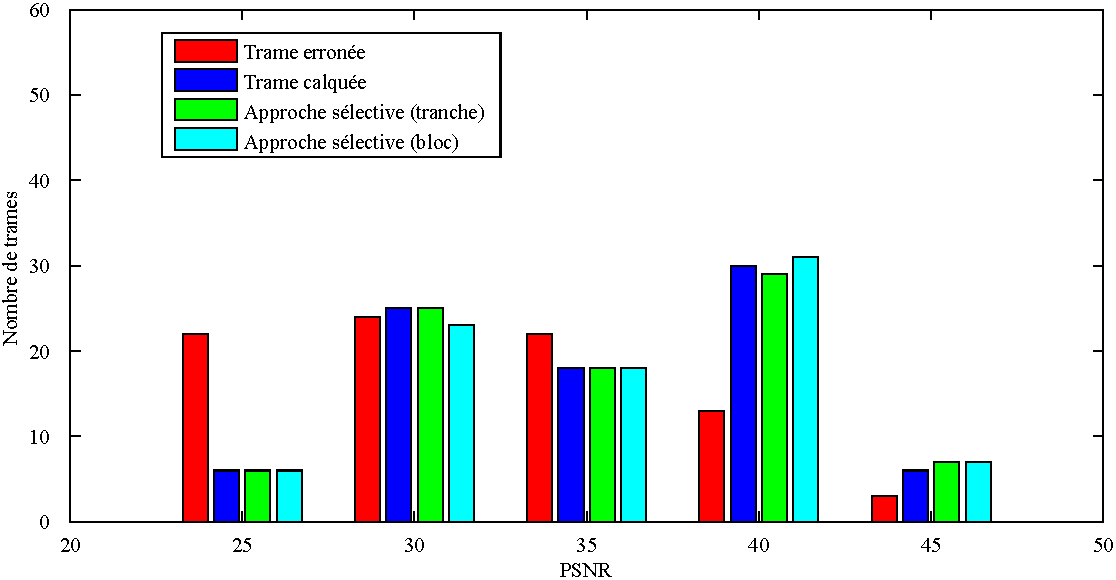
\includegraphics[width=0.97\linewidth]{Annexe/HistAllDispersed16x32.pdf} }
\caption[]{Histogrammes des PSNR des trames, selon l'approche de dissimulation
utilisée. (QP = 16, BER = 0.0032, FMO = Dispersé)}
\label{fig-HistAllDispersed16x32}
\end{figure}

\begin{figure} \fbox{ \centering
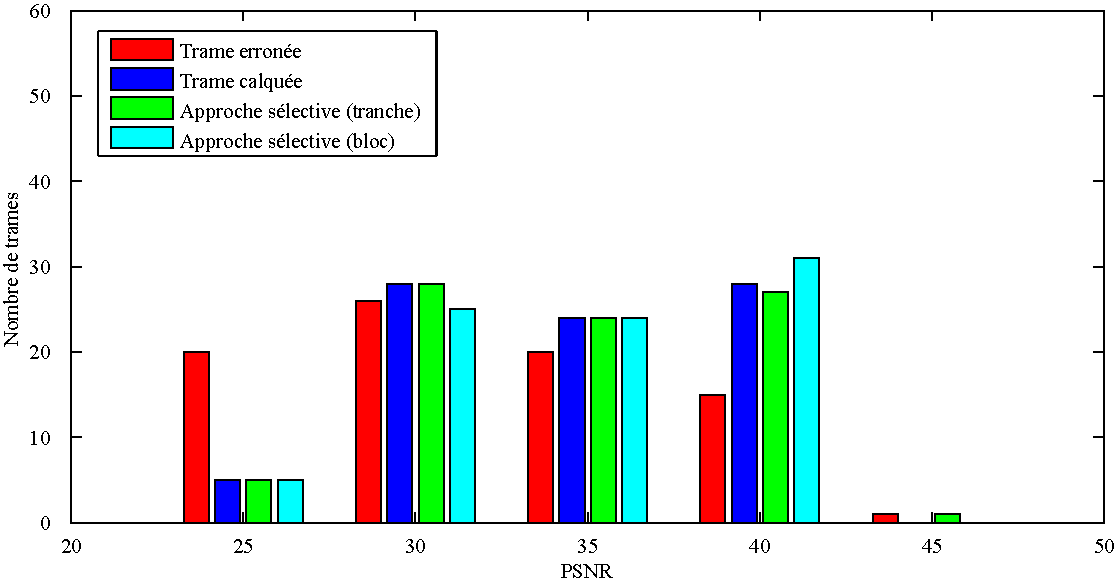
\includegraphics[width=0.97\linewidth]{Annexe/HistAllDispersed20x32.pdf} }
\caption[]{Histogrammes des PSNR des trames, selon l'approche de dissimulation
utilisée. (QP = 20, BER = 0.0032, FMO = Dispersé)}
\label{fig-HistAllDispersed20x32}
\end{figure}

\begin{figure} \fbox{ \centering
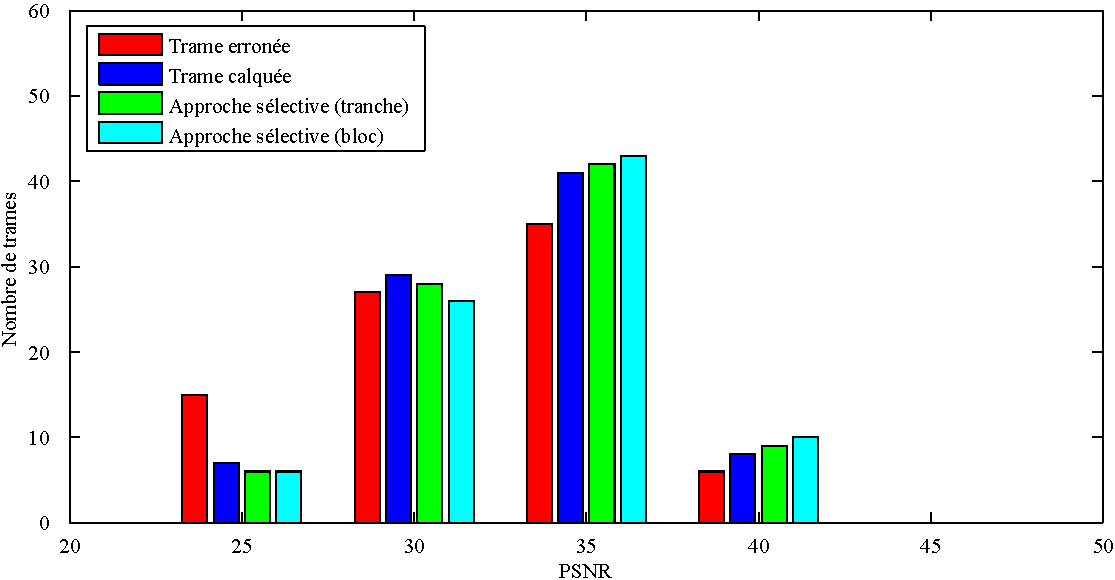
\includegraphics[width=0.97\linewidth]{Annexe/HistAllDispersed24x32.pdf} }
\caption[]{Histogrammes des PSNR des trames, selon l'approche de dissimulation
utilisée. (QP = 24, BER = 0.0032, FMO = Dispersé)}
\label{fig-HistAllDispersed24x32}
\end{figure}

\begin{figure} \fbox{ \centering
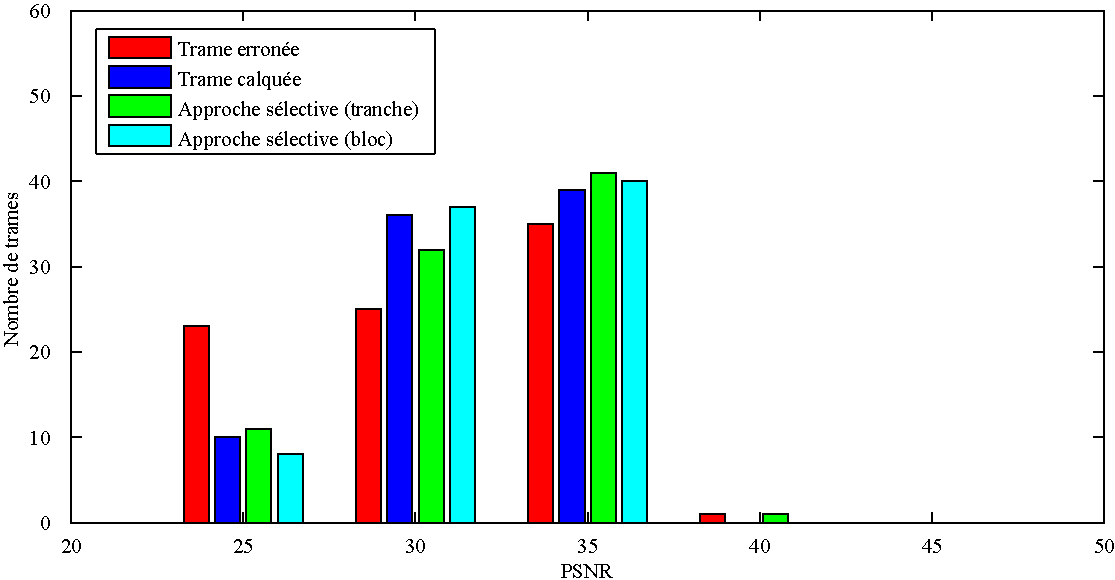
\includegraphics[width=0.97\linewidth]{Annexe/HistAllDispersed28x32.pdf} }
\caption[]{Histogrammes des PSNR des trames, selon l'approche de dissimulation
utilisée. (QP = 28, BER = 0.0032, FMO = Dispersé)}
\label{fig-HistAllDispersed28x32}
\end{figure}

\FloatBarrier
% ------------------------------------------------------------------------------
% Interleaved

\begin{table}
\caption[Résumé des résultats obtenus sur l'ensemble des séquences pour un taux
d'erreurs de 0.0032 (entrelacé)]{Résumé des résultats obtenus sur l'ensemble des
séquences pour un taux d'erreurs de 0.0032 (entrelacé).}
\centering
\begin{tabular}{| l | c | c | c | c |}
 \hline
 \multirow{2}{*}{\textbf{Approche}} & \multicolumn{4}{c |}{\textbf{PSNR Moyen
 entrelacé (dB)}}\\
  \cline{2-5}
   &QP 16 & QP 20 & QP 24 & QP 28 \\ \hline
Encodée (sans erreur) & 45.83& 42.56& 39.56& 36.85\\ \hline
Sélective par bloc (avec référence) & 39.50& 38.69& 37.51& 35.63\\
\hline Sélective par tranche (avec référence)& 39.27& 38.36& 37.07&
35.30\\ \hline Sélective par bloc & \textbf{39.14}& \textbf{38.33}&
\textbf{37.09}& \textbf{35.29}\\ \hline Sélective par tranche &
\textbf{39.13}& \textbf{38.18}& \textbf{36.85}& \textbf{35.16}\\ \hline
Dissimulation tranche calquée & 39.26& 38.14& 36.72& 34.94\\ \hline
Trame corrompue & 39.26& 38.14& 36.72& 34.94\\
\hline
\end{tabular}
\end{table}


\begin{figure} \fbox{ \centering
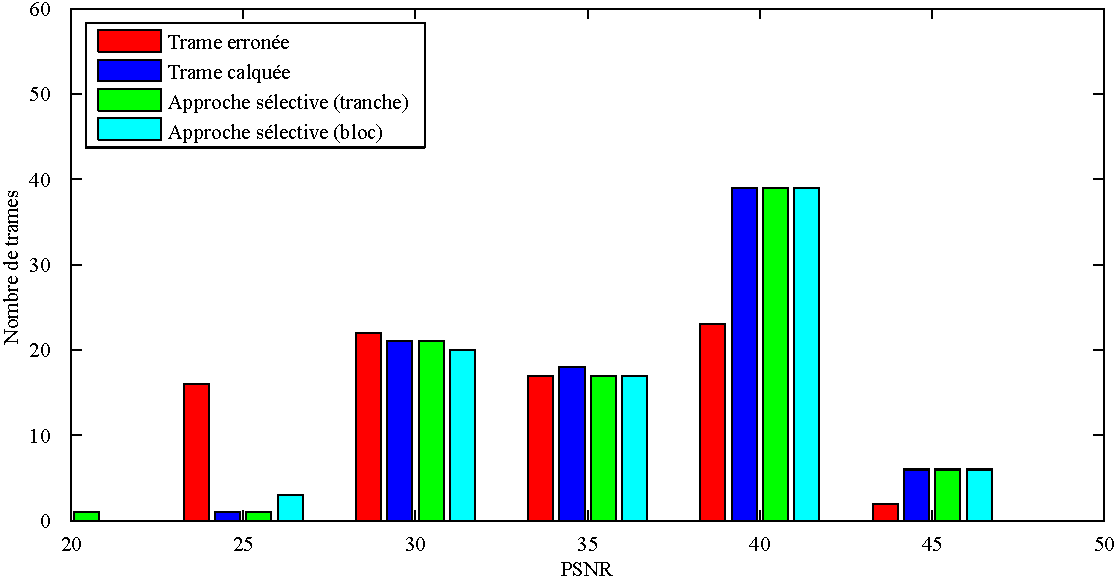
\includegraphics[width=0.97\linewidth]{Annexe/HistAllInterleaved16x32.pdf} }
\caption[]{Histogrammes des PSNR des trames, selon l'approche de dissimulation
utilisée. (QP = 16, BER = 0.0032, FMO = Entrelacé)}
\label{fig-HistAllDInterlaced16x32}
\end{figure}


\begin{figure} \fbox{ \centering
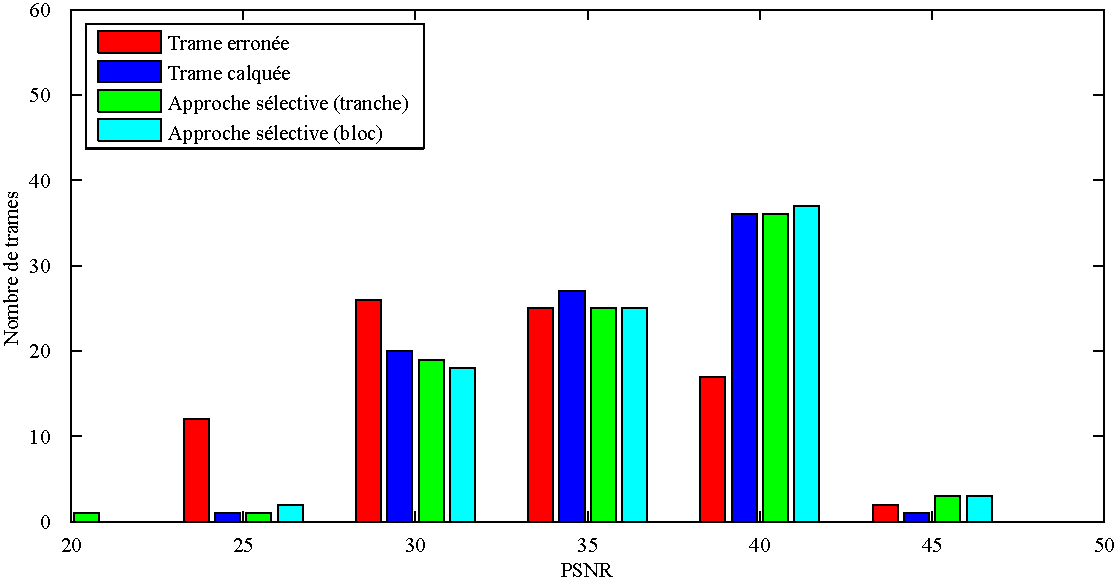
\includegraphics[width=0.97\linewidth]{Annexe/HistAllInterleaved20x32.pdf} }
\caption[]{Histogrammes des PSNR des trames, selon l'approche de dissimulation
utilisée. (QP = 20, BER = 0.0032, FMO = Entrelacé)}
\label{fig-HistAllDInterlaced20x32}
\end{figure}


\begin{figure} \fbox{ \centering
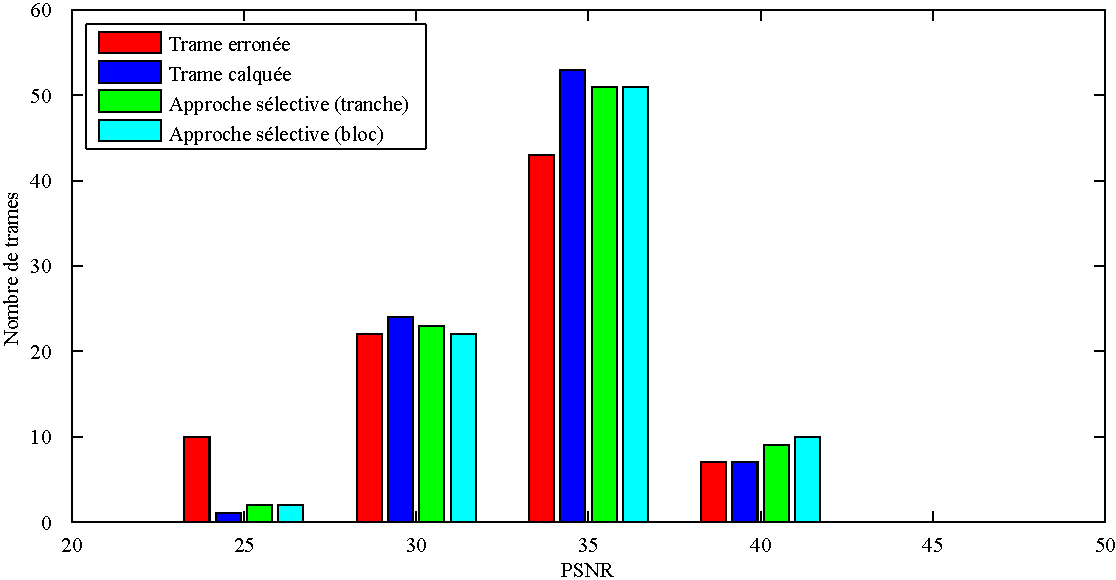
\includegraphics[width=0.97\linewidth]{Annexe/HistAllInterleaved24x32.pdf} }
\caption[]{Histogrammes des PSNR des trames, selon l'approche de dissimulation
utilisée. (QP = 24, BER = 0.0032, FMO = Entrelacé)}
\label{fig-HistAllDInterlaced24x32}
\end{figure}


\begin{figure} \fbox{ \centering
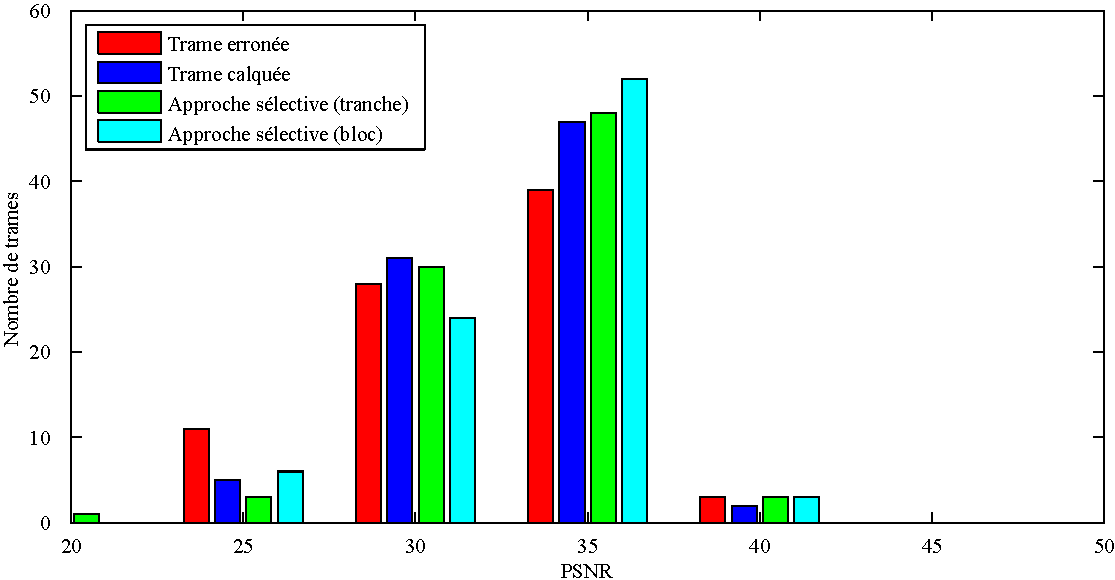
\includegraphics[width=0.97\linewidth]{Annexe/HistAllInterleaved28x32.pdf} }
\caption[]{Histogrammes des PSNR des trames, selon l'approche de dissimulation
utilisée. (QP = 28, BER = 0.0032, FMO = Entrelacé)}
\label{fig-HistAllDInterlaced28x32}
\end{figure}
\end{subsection}

\end{section}
